\chapter{Introduction}

The internet has become an integral part of modern life, connecting people all over the world and enabling access to a vast amount of information and resources. It has transformed the way we communicate, do business, and access entertainment. In addition, the internet has made it easier for people to access education, healthcare, and government services, and has helped to bridge the digital divide between those who have access to technology and those who do not.
If an area experiences a loss of connectivity due to natural disasters or lacks access to the internet, the residents of that area will be unable to utilize these services. The COVID-19 pandemic highlighted the importance of internet access as a fundamental necessity and the challenges faced by those who do not have reliable internet connections. According to a report by the United Nations (UN), the pandemic exacerbated existing inequalities and has disproportionately affected people living in rural and underserved areas, who have limited or no access to the internet~\cite{unreport}.

Delay-tolerant networks (DTNs) are a type of networking technology that can be used to deliver internet connectivity to remote areas where traditional networking infrastructure is unavailable or unreliable. DTNs are designed to operate in these environments that cannot rely on continuous connectivity ~\cite{dtn_intro}. They use a store and forward mechanism; a node receiving data from a sender stores the data and waits for a connection to be established with the recipient. When a connection is established, the node forwards the data to the recipient. This process is repeated at each intermediate node along the path until the data reaches its final destination. This allows DTNs to function in scenarios where there is a high degree of network disruption as is the case in remote, disaster-stricken areas and space communications as well.


\section{Project Overview} 

\begin{figure}[ht!]
\centering
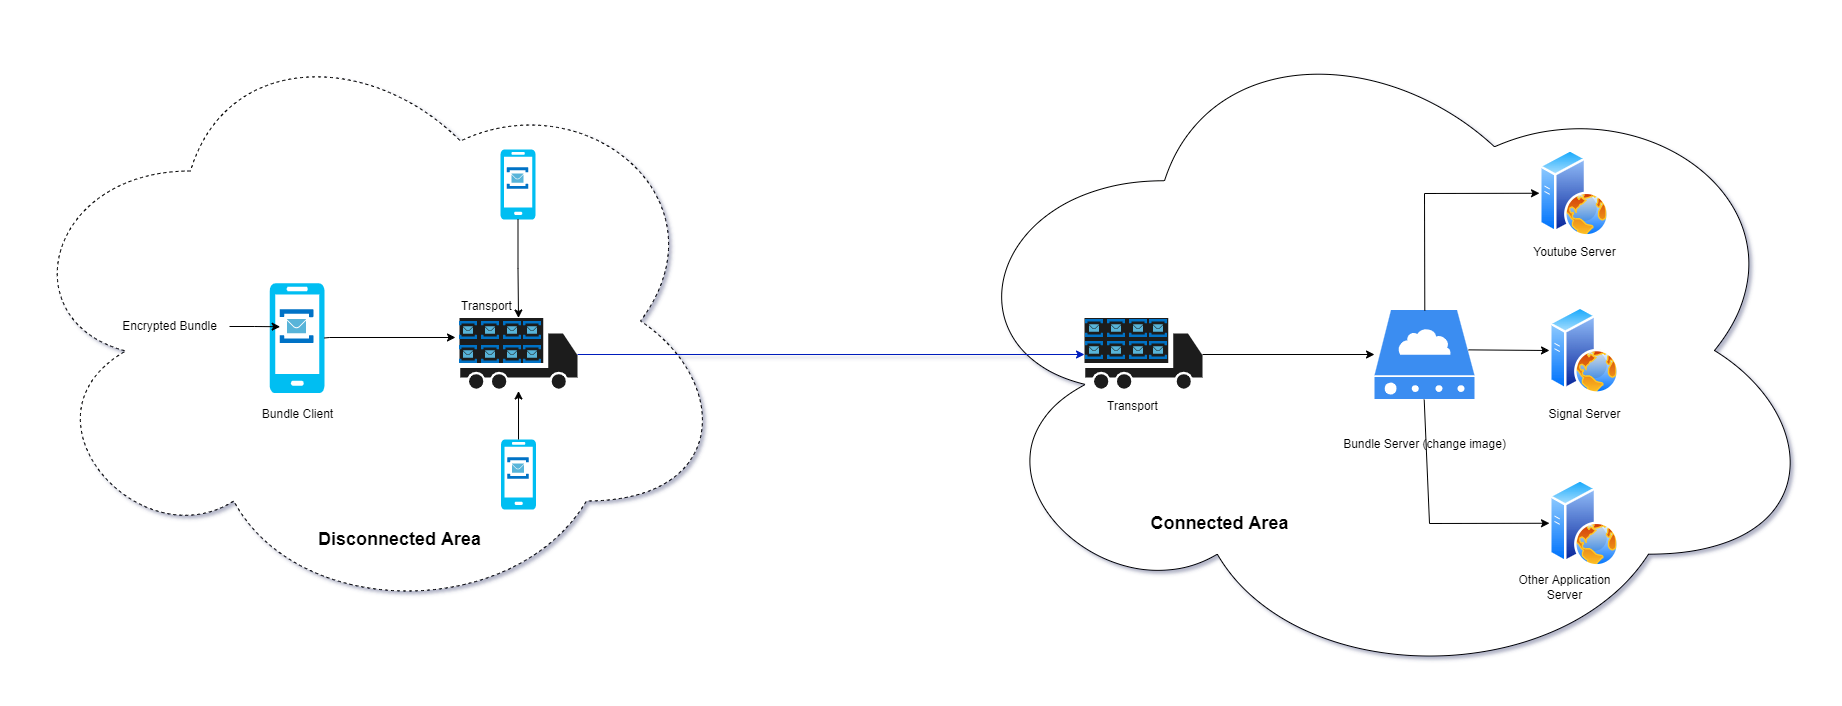
\includegraphics[width= 150mm]{./images/Introduction.png}
\caption{Project Overview}
\end{figure}

This project proposes an architecture that aims to utilize existing hardware to provide internet access to disaster-affected areas or regions with limited or no connectivity. The users can use their phones to utilize this service by downloading the respective applications from the Google Play Store. When internet connectivity is no longer available, devices can use the \textit{Bundle Client} application to access the internet for selected applications. This device will be referred to henceforth as the \textit{Bundle Client} or simply as the \textit{client}. Another mobile device that is capable of moving from a disconnected to a connected area will use the \textit{Bundle Tranport} application to store and forward bundles that it receives from clients it comes in contact with. This device will henceforth be referred to as the \textit{Bundle Tranport} or simply as the \textit{tranport}.

When a transport comes in contact with a client, the client combines data from all supported applications into a single \textit{Bundle}, encrypts it, and sends it to the \textit{Transport}. The transport stores the bundles and physically moves to another location where it can connect to the internet. The figure above illustrates this scenario. Once it reaches a connected area, it forwards all the bundles to the \textit{Bundle Server}, which is a server that is running on the cloud that accepts and processes bundles. The Bundle Server then decrypts the bundles and forwards them to the respective application servers. The response is then sent back the same path.

This solution offers a convenient way to establish connectivity in disconnected areas without the need for additional hardware. It can accommodate a wide range of application data, including those with longer half-lives. The term 'half-life' in this context refers to the amount of time it takes for the majority of the data to become irrelevant~\cite{data_halflife}. Intermediate nodes also do not need to be trusted in this case as they simply act as a forwarding medium between the client and server. All data received from the transport at either end is not trusted until it can be decrypted successfully which provides data integrity, confidentiality and authentication.